
\begin{figure*}
    \centering
    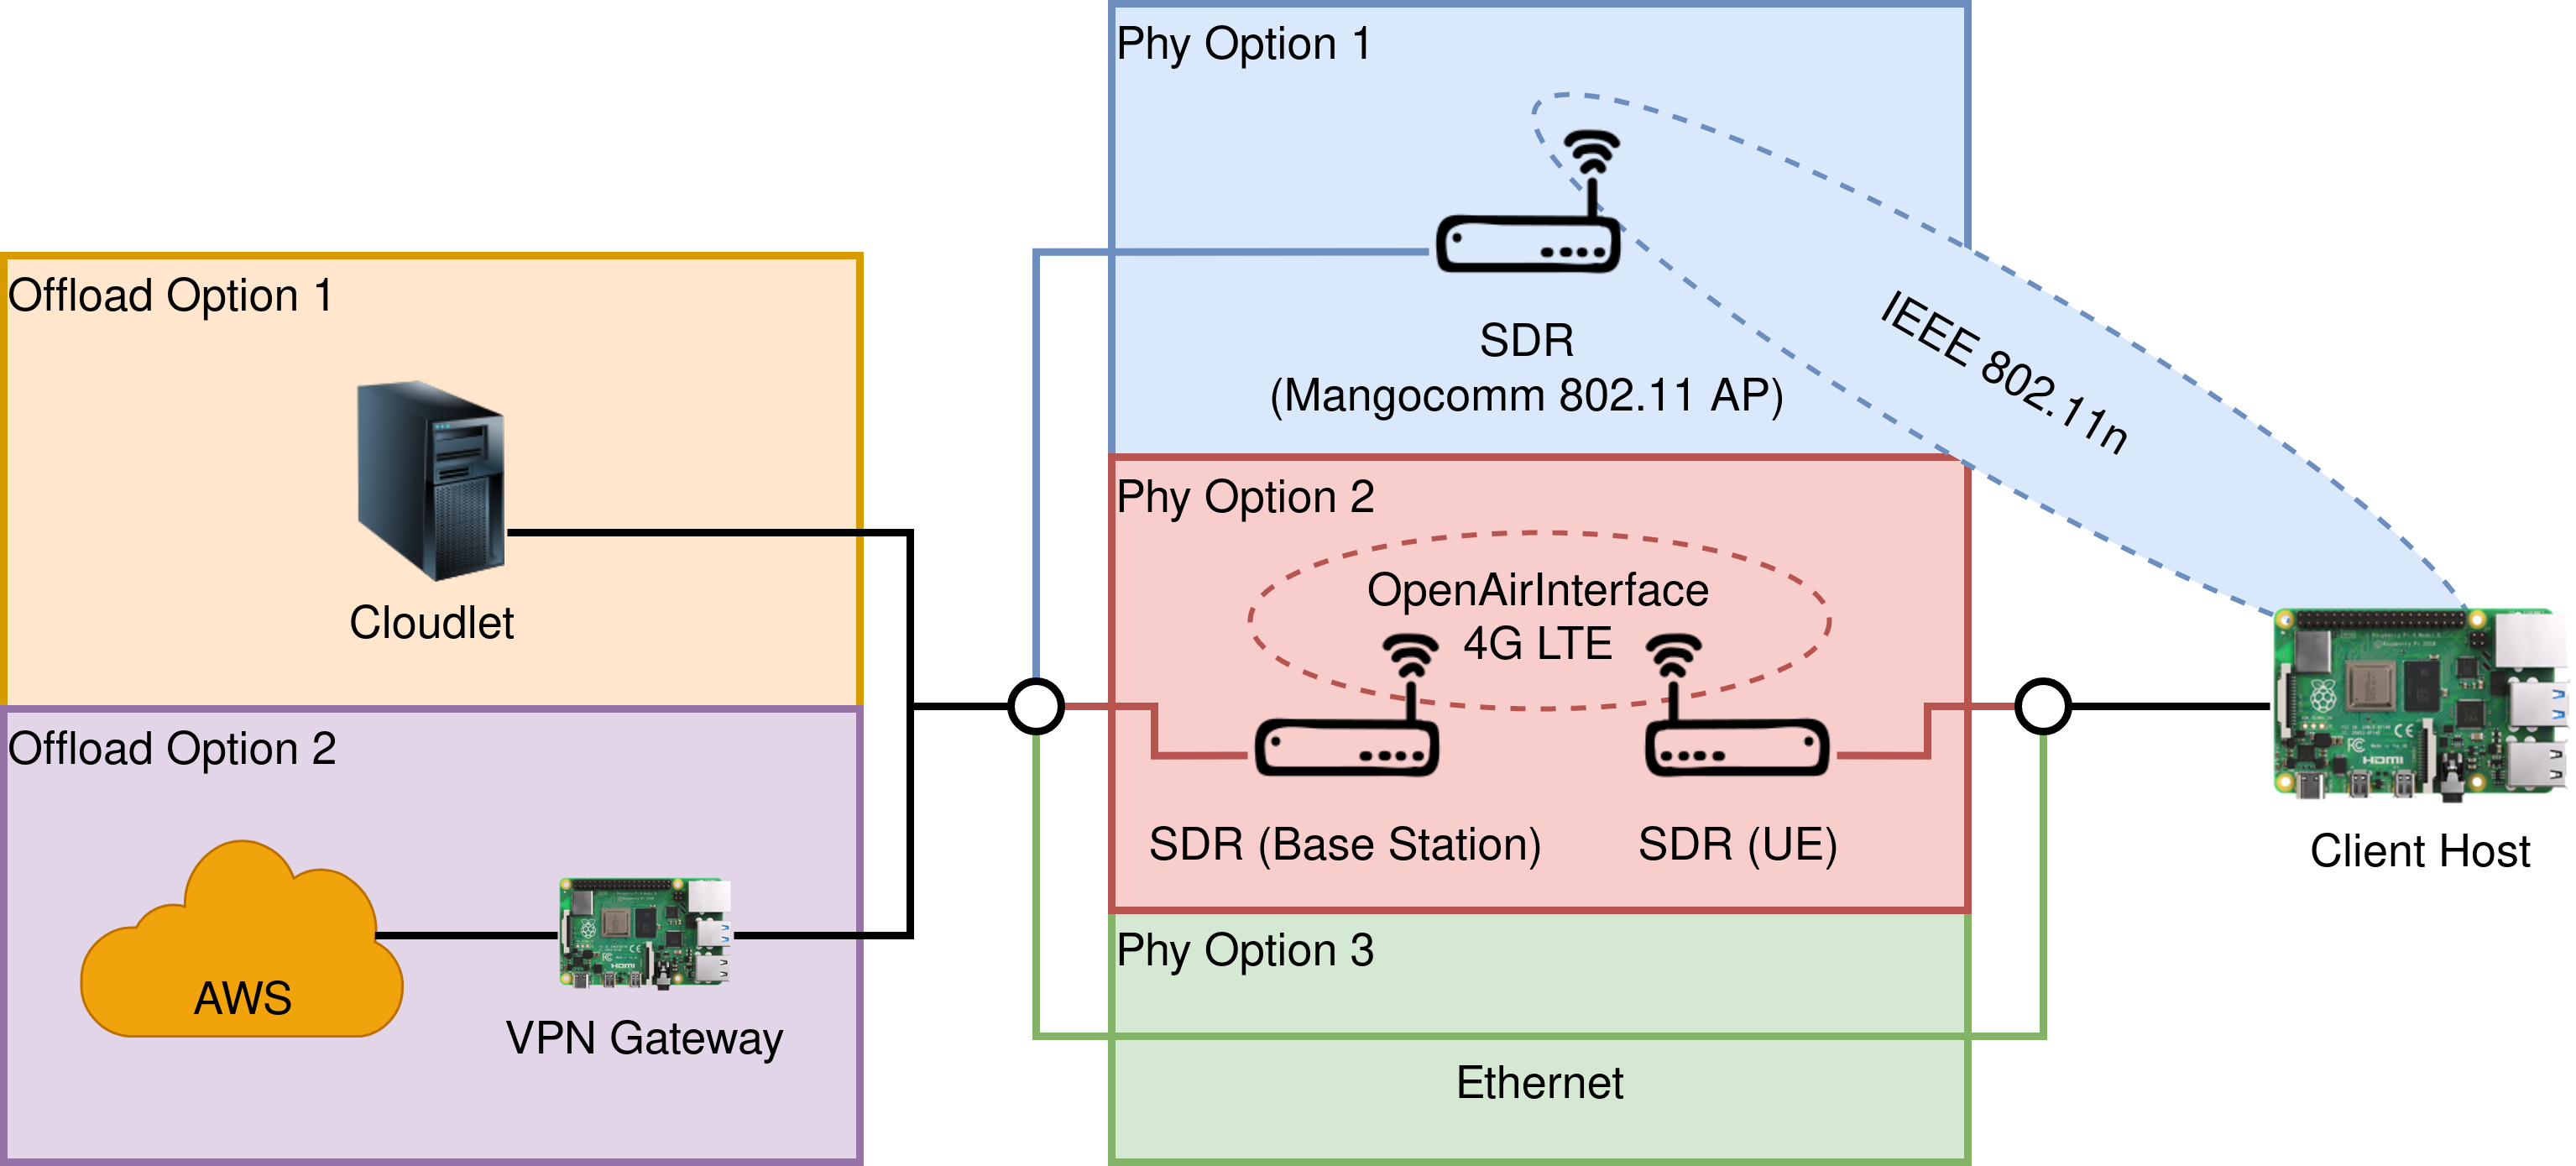
\includegraphics[width=\textwidth]{publications/2022Ainur/figures/demo_hardware}
    \caption[caption]{%
        The possible workload offloading setups and physical layer configurations used in the demo.
        Not pictured, in Phy Option 2:
        \begin{inlineenum}
            \item \gls{SDR} processing hosts
            \item additional base-station host for the Core Network and \gls{eNodeB}
        \end{inlineenum}.
    }\label{paper:olguinmunoz2022ainur:fig:democonfigs}
\end{figure*}

\begin{figure}
    \centering
    \begin{subfigure}{.45\textwidth}
        \centering
        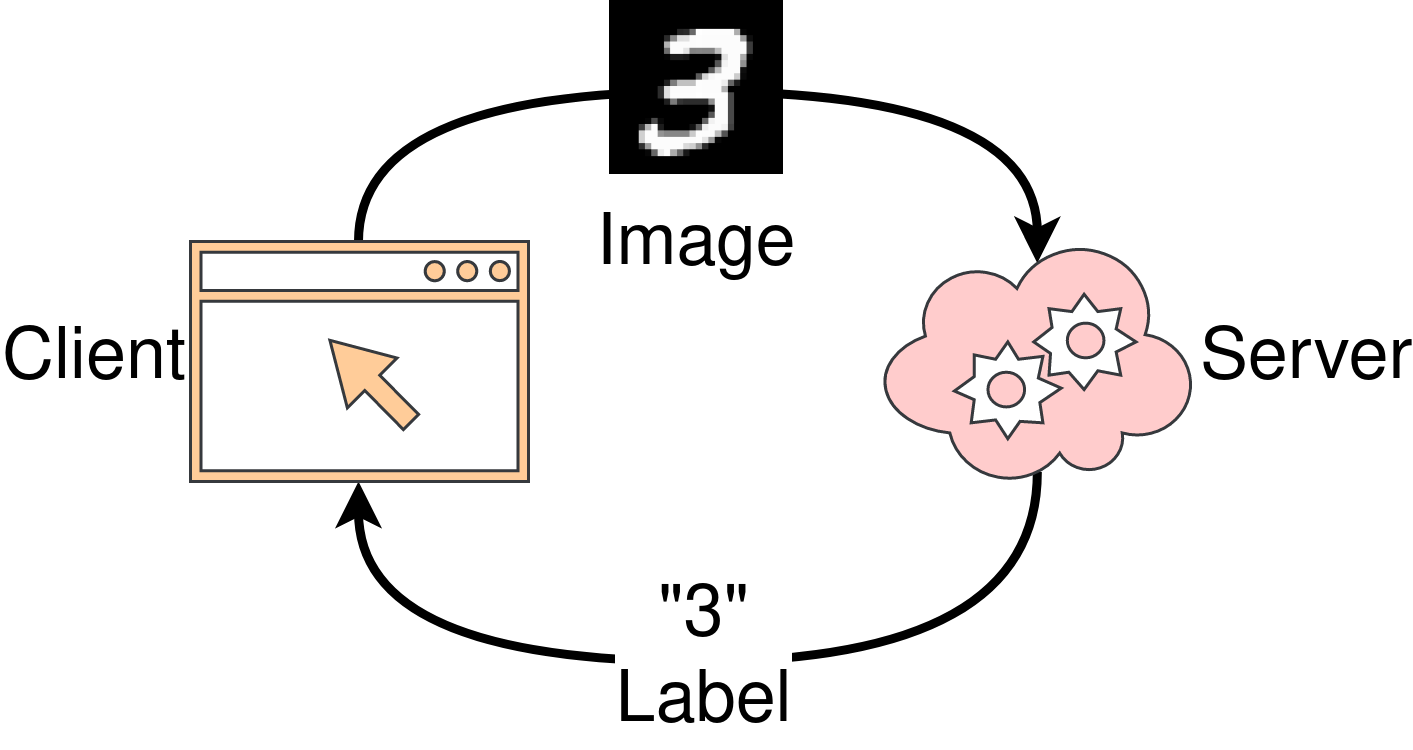
\includegraphics[width=\textwidth]{publications/2022Ainur/figures/demo_workload_1}
        \caption{Workload 1: \acs{MNIST} image classifier}\label{paper:olguinmunoz2022ainur:fig:wkld:mnist}
    \end{subfigure}%
    \hfill%
%    \vspace{1em}
    \begin{subfigure}{.45\textwidth}
        \centering
        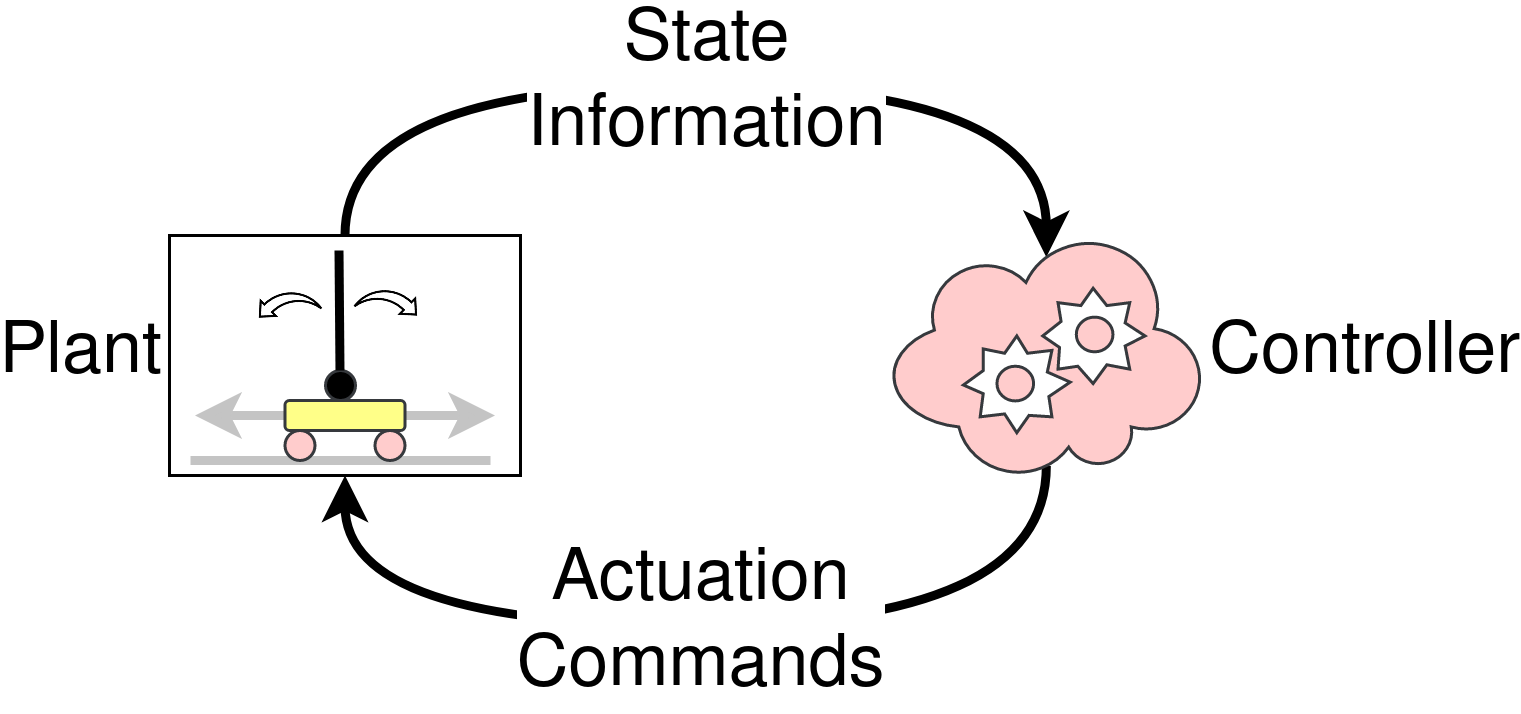
\includegraphics[width=\textwidth]{publications/2022Ainur/figures/demo_workload_2}
        \caption{Workload 2: inverted pendulum \acs{NCS}}\label{paper:olguinmunoz2022ainur:fig:wkld:ncs}
    \end{subfigure}
    \caption{Demonstration workloads}\label{paper:olguinmunoz2022ainur:fig:wkld}
\end{figure}

\section{Demo}\label{paper:olguinmunoz2022ainur:demo}

In this demo, we will show the flexibility of Ainur for running end-to-end experimental workloads on both the Edge and the Cloud.
This will be done interactively, and members of the audience will be invited to propose testbed configurations.

\Cref{paper:olguinmunoz2022ainur:fig:democonfigs} illustrates the possible configurations for the testbed.
Workloads are deployed on client hosts, and computation is offloaded either to an edge server (cloudlet), or to \gls{AWS} \gls{EC2} instances on the cloud.
Communication between the client- and server-sides of the workload will occur over one of three possible physical link layer setups:
\begin{description}
    \item[Wi-Fi:] \pgls{SDR} is configured as an IEEE 802.11n access point, and client hosts connect to it using on-board Wi-Fi.
    \item[4G \gls{LTE}:] \pgls{SDR} is configured as an 4G \gls{LTE} base station, and another is configured as an 4G \gls{LTE} \gls{UE}.
    Together these radios act as an \gls{LTE} bridge between the client-side and the server-side of the network, and all client-server traffic is routed through them.
    \item[Ethernet:] connects everything through plain ethernet.
\end{description}

The number of workload instances (and therefore client hosts) deployed in each execution of this demonstration will range from \numrange[]{1}{10}.
Workloads deployed to the cloud will be able to target any of \gls{AWS}'s datacenters.

We will employ two different workloads for this demonstration, illustrated in \cref{paper:olguinmunoz2022ainur:fig:wkld}.
The first of these (\cref{paper:olguinmunoz2022ainur:fig:wkld:mnist}) consists of a proof-of-concept web application which implements a simple classifier to identify hand-drawn digits from the widely-used \gls{MNIST} dataset~\cite{deng2012mnist}.
The application consists of a client with a web interface, and \pgls{HTTP} server which responds to requests from the client and performs the actual image recognition.
This workload is intended to showcase in an interactive manner the effects of placing computation at different points of the network, and how Ainur simplifies these deployments.

The second workload (\cref{paper:olguinmunoz2022ainur:fig:wkld:ncs}) corresponds to \pgls{NCS} balancing an inverted pendulum, implemented on a software framework for the emulation of \glspl{NCS} using cloud-native technologies~\cite{olguinmunoz2022cleave}.
It consists of an emulation of the physical inverted pendulum system plant and a software-implemented proportional-differential controller.
These components communicate with each other over the \gls{UDP}.
This workload will be used to showcase the utility of Ainur for automating the execution of batches of experiments potentially including multiple different clients, servers, and physical layers.

\subsection{Testbed Setup}

This demonstration will be performed on a testbed consisting of
\begin{inlineenum}[itemjoin={{; }}, itemjoin*={{; and finally }}]
    \item \num{10} Raspberry Pi 4 Model B boards, acting as client-side workload hosts
    \item a Raspberry Pi 4 Model B acting as \gls{VPN} gateway for the workload network
    \item a Raspberry Pi 4 Model B acting as \gls{VPN} gateway for the management network, as well as hosting the necessary \gls{NTP} and \gls{DNS} server software
    \item a \texttt{i386} workstation, acting as an edge-side workload host
    \item a configurable number of  \gls{AWS} \gls{EC2} cloud instances acting as cloud servers
    \item a separate \texttt{i386} workstation hosting the Fluent server and on which Ainur is deployed as well.
\end{inlineenum}
These nodes are interconnected using a combination of managed switches, \glspl{SDR}, and \gls{VPN} gateways; please refer to \cref{paper:olguinmunoz2022ainur:fig:network} for an architectural overview of this setup.


\subsection{Demo Procedure}

\subsubsection{Workload 1}

\begin{figure}
    \centering
    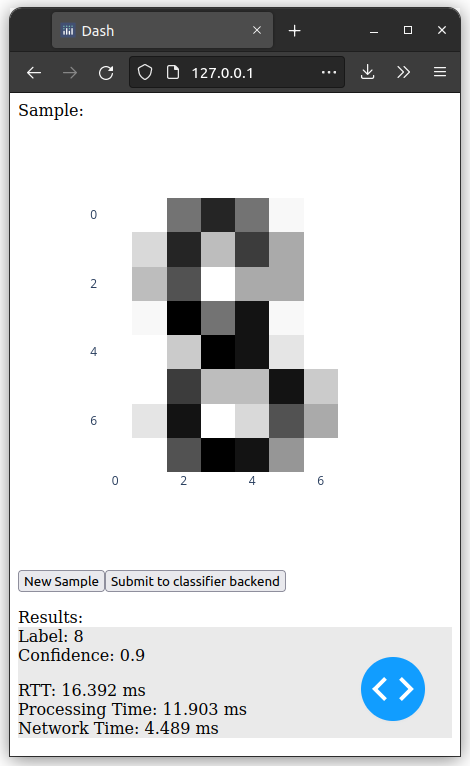
\includegraphics[height=25em]{publications/2022Ainur/figures/demo_mockup}
    \caption{Screenshot of the user interface of demo workload 1. After deciding on the placement of the compute backend and the type of physical layer connecting client and backend, participants will use this interface to interact with the system.}\label{paper:olguinmunoz2022ainur:fig:mockup}
\end{figure}

Participants will be asked to choose
\begin{inlineenum}
    \item a location to offload computation to (local (i.e.\ no offloading), edge, or any \gls{AWS} datacenter)
    \item a physical layer for the first hop of the network (Wi-Fi, 4G \gls{LTE}, or ethernet).
\end{inlineenum}
Through the Ainur command line, we will deploy a single client-server pair according to the specifications.
Next, participants will be able to access the client web interface and interact with the server by requesting classification of images from the \gls{MNIST} database.
The server will respond to these, and the assigned labels will be visible on the web interface together with timing statistics for each request, see \cref{paper:olguinmunoz2022ainur:fig:mockup}.

\subsubsection{Workload 2}

Participants will be asked to specify the full, arbitrarily complex, experimental scenario, including the number of clients, physical layers (single or multiple, and which clients are on each physical link), and offloading configuration (number of instances on the edge vs.\ on the cloud, which \gls{AWS} datacenters to deploy to).
Configuration will be specified through a \gls{YAML} file, which will then be parsed by Ainur for the automatic execution of the scenario.
